% vim: ts=4 sts=4 sw=4 et tw=75
\chapter{Performance}
\label{chap:performance}
\begin{quote}
    His promises were, as he then was, mighty; But his performance, as he
    is now, nothing.
\end{quote}
\begin{quotesrc}
    Shakespeare, \bookname{King Henry VIII}
\end{quotesrc}

Long ago, programmers went to great effort to make their programs efficient
because computers were slow and expensive. Today, machines are much cheaper
and faster, so the need for absolute efficiency is greatly reduced. Is it
still worth worrying about performance?

Yes, but only if the problem is important, the program is genuinely too
slow, and there is some expectation that it can be made faster while
maintaining correctness, robustness, and clarity. A fast program that gets
the wrong answer doesn't save any time.

Thus the first principle of optimization is don't. Is the program good
enough already? Knowing how a program will be used and the environment it
runs in, is there any benefit to making it faster? Programs written for
assignments in a college class are never used again; speed rarely matters.
Nor will speed matter for most personal programs, occasional tools, test
frameworks, experiments, and prototypes. The run-time of a commercial
product or a central component such as a graphics library can be critically
important, however, so we need to understand how to think about performance
issues.

When should we try to speed up a program? How can we do so? What can we
expect to gain? This chapter discusses how to make programs run faster or
use less memory. Speed is usually the most important concern, so that is
mostly what we'll talk about. Space (main memory, disk) is less frequently
an issue but can be crucial, so we will spend some time and space on that
too.

As we observed in Chapter \ref{chap:alds}, the best strategy is to use the
simplest, cleanest algorithms and data structures appropriate for the task.
Then measure performance to see if changes are needed; enable compiler
options to generate the fastest possible code; assess what changes to the
program itself will have the most effect; make changes one at a time and
re-assess; and keep the simple versions for testing revisions against.

Measurement is a crucial component of performance improvement since
reasoning and intuition are fallible (易错的) guides and must be
supplemented with tools like timing commands and profilers (探查).
Performance improvement has much in common with testing, including such
techniques as automation, keeping careful records, and using regression
(回归) tests to make sure that changes preserve correctness and do not undo
previous improvements.

If you choose your algorithms wisely and write well originally you may find
no need for further speedups. Often minor changes will fix any performance
problems in well-designed code, while badly-designed code will require
major rewriting.

\section{A Bottleneck}
\label{sec:bootleneck}
Let us begin by describing how a bottleneck was removed from a critical
program in our local environment.

Our incoming mail funnels (漏斗) through a machine, called a gateway, that
connects our internal network with the external Internet. Electronic mail
messages from outside -- tens of thousands a day for a community of a few
thousand people -- arrive at the gateway and are transferred to the
internal network; this separation isolates our private network from the
public Internet and allows us to publish a single machine name (that of the
gateway) for everyone in the community.

One of the services of the gateway is to filter out "spam (罐头猪肉)."
unsolicited (未经同意的) mail that advertises services of dubious (可疑的)
merit (值得). After successful early trials of the spam filter, the service
was installed as a permanent feature for all users of the mail gateway, and
a problem immediately became apparent. The gateway machine, antiquated
(老旧的) and already very busy, was overwhelmed (倾覆) because the
filtering program was taking so much time -- much more time than was
required for all the other processing of each message -- that the mail
queues filled and message delivery was delayed by hours while the system
struggled to catch up.

This is an example of a true performance problem: the program was not fast
enough to do its job, and people were inconvenienced by the delay. The
program simply had to run much faster.

Simplifying quite a bit, the spam filter runs like this. Each incoming
message is treated as a single string, and a textual pattern matcher
examines that string to see if it contains any phrases from known spam,
such as "Make millions in your spare time" or "XXX-rated." Messages tend to
recur (重发), so this technique is remarkably effective, and if a spam
message is not caught, a phrase is added to the list to catch it next time.

None of the existing string-matching tools, such as \verb'grep', had the
right combination of performance and packaging (封装), so a special-purpose
spam filter was written. The original code was very simple; it looked to
see if each message contained any of the phrases (patterns):
\begin{wellcode}
    /* isspam: test mesg for occurrence of any pat */
    int isspam(char *mesg)
    {
        int i;

        for (i = 0; i < npat; i++)
            if (strstr(mesg, pat[i]) != NULL) {
                printf("spam: match for '%s'\n", pat[i]);
                return 1;
            }

        return 0;
    }
\end{wellcode}
How could this be made faster? The string must be searched, and the
\verb'strstr' function from the C library is the best way to search: it's
standard and efficient.

\emph{Using profiling (靠模切削),} a technique we'll talk about in the next
section, it became clear that the implementation of \verb'strstr' had
unfortunate properties when used in a spam filter. By changing the way
\verb'strstr' worked, it could be made more efficient \emph{for this
    particular problem}.

The existing implementation of \verb'strstr' looked something like this:
\begin{wellcode}
    /* simple strstr: use strchr to look for first character */
    char *strstr(const char *s1, const char *s2)
    {
        int n;

        n = strlen(s2);
        for (;;) {
            s1 = strchr(s1, s2[0]);
            if (s1 == NULL)
                return NULL;
            if (strncmp(s1, s2, n) == 0)
                return s1;
            s1++;
        }
    }
\end{wellcode}
It had been written with efficiency in mind, and in fact for typical use it
was fast because it used highly-optimized library routines to do the work.
It called \verb'strchr' to find the next occurrence of the first character
of the pattern, and then called \verb'strncmp' to see if the rest of the
string matched the rest of the pattern. Thus it skipped quickly over most
of the message looking for the first character of the pattern.  and then
did a fast scan to check the rest. Why would this perform badly?

There are several reasons. First, strncmp takes as an argument the length
of the pattern. which must be computed with \verb'strlen'. But the patterns
are fixed, so it shouldn't be necessary to recompute their lengths for each
message.

Second, \verb'strncmp' has a complex inner loop. It must not only compare
the bytes of the two strings, it must look for the terminating \verb'\0'
byte on both strings while also counting down the length parameter. Since
the lengths of all the strings are known in advance (though not to
strncmp), this complexity is unnecessary; we know the counts are right so
checking for the \verb'\n' wastes time.

Third, \verb'strchr' is also complex, since it must look for the character
and also watch for the \verb'\0' byte that terminates the message. For a
given call to \verb'isspam', the message is fixed, so time spent looking
for the \verb'\0' is wasted since we know where the message ends.

Finally, although \verb'strncmp', \verb'strchr' , and \verb'strlen' are all
efficient in isolation, the overhead of calling these functions is
comparable to the cost of the calculation they will perform. It's more
efficient to do all the work in a special, carefully written version of
\verb'strstr' and avoid calling other functions altogether.

These sorts of problems are a common source of performance trouble -- a
routine or interface works well for the typical case, but performs poorly
in an unusual case that happens to be central to the program at issue. The
existing \verb'strstr' was fine when both the pattern and the string were
short and changed each call, but when the string is long and fixed, the
overhead is prohibitive (可抑制的).

With this in mind, \verb'strstr' was rewritten to walk the pattern and
message strings together looking for matches, without calling subroutines.
The resulting implementation has predictable behavior: it is slightly
slower in some cases, but much faster in the spam filter and, most
important, is never terrible. To verify the new implementation's
correctness and performance, a performance test suite was built.  This
suite included not only simple examples like searching for a word in a
sentence, but also pathological (病态的) cases such as looking for a
pattern of a single x in a string of a thousand e's and a pattern of a
thousand x's in a string of a single e, both of which can be handled badly
by naive implementations. Such extreme cases are a key part of performance
evaluation.

The library was updated with the new \verb'strstr' and the spam filter ran
about $30\%$ faster, a good payoff for rewriting a single routine.

Unfortunately, it was still too slow.

When solving problems, it's important to ask right question. Up to now,
we've been asking for the fastest way to search for a textual pattern in a
string. But the real problem is to search for a large, fixed set of textual
patterns in a long, variable string. Put that way, \verb'strstr' is not so
obviously the right solution.

The most effective way to make a program faster is to use a better
algorithm.  With a clearer idea of the problem, it's time to think about
what algorithm would work best.

The basic loop,
\begin{wellcode}
    for (i = 0; i < npat; i++)
        if (strstr(mesg, pat[i]) != NULL)
            return 1;
\end{wellcode}
scans down the message \verb'npat' independent times; assuming it doesn't
find any matches, it examines each byte of the message \verb'npat' times,
for a total of \verb'strlen(mesg)*npat' comparisons.

A better approach is to invert the loops, scanning the message once in the
outer loop while searching for all the patterns in parallel in the inner loop:
\begin{wellcode}
    for (j = 0; mesg[j] != '\0'; j++)
        if (some pattern matches starting at mesg[j])
            return 1;
\end{wellcode}
The performance improvement stems from (主要来源于) a simple observation.
To see if any pattern matches the message at position \verb'j', we don't
need to look at all patterns, only those that begin with the same character
as \verb'mesg[j]'. Roughly, with 52 upper and lower-case letters we might
expect to do only \verb'strlen(mesg)*npat/52' comparisons. Since the
letters are not evenly distributed -- words with \verb's' more often than
\verb'x' -- we won't see a factor of 52 improvement, but we should see
some. In effect, we construct a hash table using the first character of the
pattern as the key.

Given some precomputation to construct a table of which patterns begin with
each character, \verb'isspam' is still short:
\begin{wellcode}
    int patlen[NPAT];                   /* length of pattern */
    int starting[UCHAR_MAX+1][NSTART];  /* pats starting with char */
    int nstarting[UCHAR_MAX+1];         /* number of such patterns */
    ...
    /* isspam: test mesg for occurrence of any pat */
    int isspam(char *mesg)
    {
        int i, j, k;
        unsigned char c;

        for (j = 0; (c = mesg[j]) != '\0'; j++) {
            for (i = 0; i < nstarting[c]; i++) {
                k = starting[c][i];
                if (memcmp(mesg+j, pat[k], patlen[k]) == 0) {
                    printf("spam: match for '%s'\n", pat[k]);
                    return 1;
                }
            }
        }
        return 0;
    }
\end{wellcode}
The two-dimensional array \verb'starting[c][]' stores, for each character
\verb'c', the indices of those patterns that begin with that character. Its
companion \verb'nstarting[c]' records how many patterns begin with
\verb'c'. Without these tables, the inner loop would run from 0 to
\verb'npat', about a thousand; instead it runs from 0 something like 20.
Finally, the array element \verb'patlen[k]' stores the precomputed result
of \verb'strlen(pat[k])'.

The following figure sketches (概括) these data structures for a set of
three pattern that begin with the letter \verb'b':
\begin{figure}[h]
\centering
\begin{varwidth}[t]{\textwidth}
    \vspace{0pt}
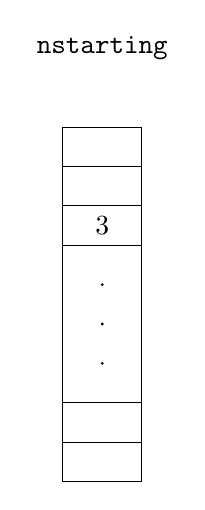
\begin{tikzpicture}
\draw (0, 0) -- (1, 0);
\draw (0, 4.5) -- (1, 4.5);
\draw (0, 0) -- (0, 4.5);
\draw (1, 0) -- (1, 4.5);

\draw (0, 3.0) -- (1, 3.0);
\draw (0, 3.5) -- (1, 3.5);
\draw (0, 4.0) -- (1, 4.0);
\node at (0.5, 3.25) {3};

\fill (0.5, 1.5) circle (0.02);
\fill (0.5, 2.0) circle (0.02);
\fill (0.5, 2.5) circle (0.02);

\draw (0, 0.5) -- (1, 0.5);
\draw (0, 1.0) -- (1, 1.0);

\node at (0.5, 5.5) {\texttt{nstarting}};
\end{tikzpicture}
\end{varwidth}
\qquad
\begin{varwidth}[t]{\textwidth}
    \vspace{0pt}
\begin{tikzpicture}
\draw (0, 0) -- (3, 0);
\draw (0, 4.5) -- (3, 4.5);
\draw (0, 0) -- (0, 4.5);
\draw (3, 0) -- (3, 4.5);

\draw (0, 3.5) -- (3, 3.5);
\draw (0, 3.0) -- (3, 3.0);

\draw (0.5, 3.0) -- (0.5, 3.5);
\draw (1.0, 3.0) -- (1.0, 3.5);
\draw (1.5, 3.0) -- (1.5, 3.5);
\node at (0.25, 3.25) {17};
\node at (0.75, 3.25) {35};
\node at (1.25, 3.25) {97};
\node at (-0.7, 3.25) {\verb"['b']"};

\node at (1.5, 5.5) {\texttt{starting}};
\end{tikzpicture}
\end{varwidth}
\qquad
\begin{varwidth}[t]{\textwidth}
    \vspace{0pt}
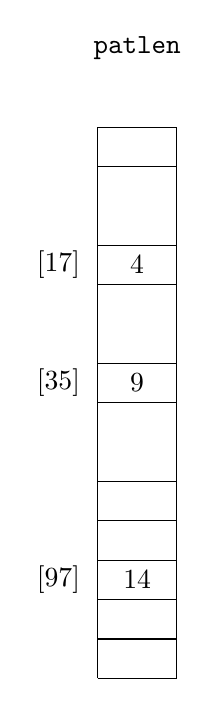
\begin{tikzpicture}
\foreach \y in {0.0, 0.5, 1.0, 1.5, 2.0, 2.5, 3.5, 4.0, 5.0, 5.5, 6.5,
	7.0} {
    \draw (0, \y) -- (1, \y);
}
\draw (0, 0) -- (0, 7.0);
\draw (1, 0) -- (1, 7.0);

\node at (0.5, 1.25) {14};
\node at (0.5, 3.75) {9};
\node at (0.5, 5.25) {4};
\node at (-0.5, 1.25) {[97]};
\node at (-0.5, 3.75) {[35]};
\node at (-0.5, 5.25) {[17]};

\node at (0.5, 8.0) {\texttt{patlen}};
\end{tikzpicture}
\end{varwidth}
\qquad
\begin{varwidth}[t]{\textwidth}
    \vspace{0pt}
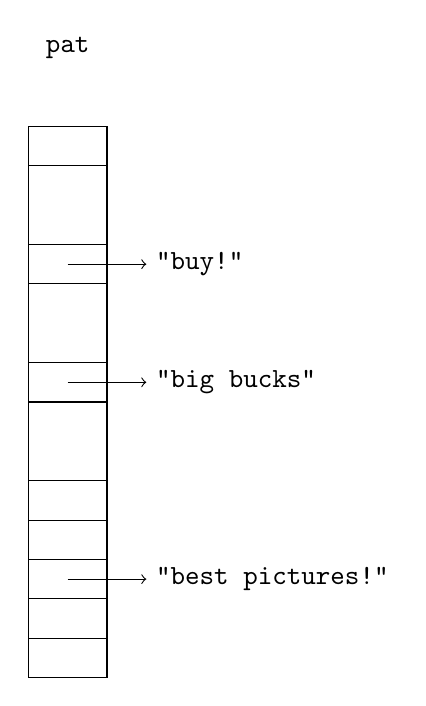
\begin{tikzpicture}
\foreach \y in {0.0, 0.5, 1.0, 1.5, 2.0, 2.5, 3.5, 4.0, 5.0, 5.5, 6.5,
	7.0} {
    \draw (0, \y) -- (1, \y);
}
\draw (0, 0) -- (0, 7.0);
\draw (1, 0) -- (1, 7.0);

\draw[->] (0.5, 1.25) -- (1.5, 1.25);
\draw[->] (0.5, 3.75) -- (1.5, 3.75);
\draw[->] (0.5, 5.25) -- (1.5, 5.25);
\node[right] at (1.5, 1.25) {\verb'"best pictures!"'};
\node[right] at (1.5, 3.75) {\verb'"big bucks"'};
\node[right] at (1.5, 5.25) {\verb'"buy!"'};

\node at (0.5, 8.0) {\texttt{pat}};
\end{tikzpicture}
\end{varwidth}

\end{figure}

The code to build these tables is easy:
\begin{wellcode}
    int i;
    unsigned char c;

    for (i = 0; i < npat; i++) {
        c = pat[i][0];
        if (nstarting[c] >= NSTART)
            printf("too many patterns (>=%d) begin '%c'",
                    NSTART, c);
        starting[c][nstarting[c]++] = i;
        patlen[i] = strlen(pat[i]);
    }
\end{wellcode}

Depending on the input, the spam filter is now five to ten times faster
than it was using the improved \verb'strstr', and seven to fifteen times
faster than the original implementation. We didn't get a factor of 52,
partly because of the non-uniform distribution of letters, partly because
the loop is more complicated in the new program, and partly because there
are still many failing string comparisons to execute, but the spam filter
is no longer the bottleneck for mail delivery. Performance problem solved.

The rest of this chapter will explore the techniques used to discover
performance problems, isolate the slow code. and speed it up. Before moving
on, though, it's worth looking back at the spam filter to see what lessons
it teaches. Most important, make sure performance matters. It wouldn't have
been worth all the effort if spam filtering wasn't a bottleneck. Once we
knew it was a problem, we used profiling and other techniques to study the
behavior and learn where the problem really lay. Then we made sure we were
solving the right problem, examining the overall program rather than just
focusing on \verb'strstr', the obvious but incorrect suspect. Finally, we
solved the correct problem using a better algorithm, and checked that it
really was faster. Once it was fast enough, we stopped; why over-engineer?

\begin{exercise}
    A table that maps a single character to the set of patterns that begin
    with that character gives an order of magnitude (巨大的) improvement.
    Implement a version of \verb'isspam' that uses two characters as the
    index. How much improvement does that lead to? These are simple special
    cases of a data structure called a trie. Most such data structures are
    based on trading (交易) space for time.
\end{exercise}

\section{Timing and Profiling}
\emph{Automate timing measurements.} Most systems have a command to measure
how long a program takes. On Unix, the command is called \verb'time':
\begin{wellcode}
    % time slowprogram
    real    7.0
    user    6.2
    sys     0.1
    %
\end{wellcode}
This runs the command and reports three numbers, all in seconds: "real"
time, the elapsed time for the program to complete; "user" CPU time, time
spent executing the user's program; and "system" CPU time, time spent
within the operating system on the program's behalf. If your system has a
similar command, use it; the numbers will be more informative, reliable,
and easier to track than time measured with a stopwatch. And keep good
notes. As you work on the program, making modifications and measurements,
you will accumulate a lot of data that can become confusing a day or two
later. (Which version was it that ran $20\%$ faster?) Many of the
techniques we discussed in the chapter on testing can be adapted for
measuring and improving performance. Use the machine to run and measure
your test suites and, most important, use regression (回归) testing to make
sure your modifications don't break the program.

If your system doesn't have a \verb'time' command, or if you're timing a
function in isolation, it's easy to construct a timing scaffold (脚手架)
analogous to a testing scaffold. C and C++ provide a standard routine,
clock, that reports how much CPU time the program has consumed so far. It
can be called before and after a function to measure CPU usage:
\begin{wellcode}
    #include <time.h>
    #include <stdio.h>
        ...
        clock_t before;
        double  elapsed;

        before = clock();
        long_running_function();
        elapsed = clock() - before;
        printf("function used %.3f seconds\n",
                elapsed / CLOCKS_PER_SEC);
\end{wellcode}
The scaling (定比) term, \verb'CLOCKS_PER_SEC', records the resolutions of the
timer as reported by clock. If the function takes only a small fraction of
a second, run it in a loop, but be sure to compensate (补偿) for loop
overhead if that is significant:
\begin{wellcode}
    before = clock();
    for (i = 0; i < 1000; i++)
        short_running_function();
    elapsed = (clock(0 - before) / (double)i;
\end{wellcode}
In Java, functions in the \verb'Date' class give wall clock time, which is
an approximation to CPU time:
\begin{wellcode}
    Date before = new Date();
    long_running_function();
    Date after = new Date();
    long elapsed = after.getTime() - before.getTime();
\end{wellcode}
The return value of \verb'getTime' is in milliseconds.

\emph{Use a profiler (刻画器).} Besides a reliable timing method, the most
important tool for performance analysis is a system for generating
profiles. A prqfile is a measurement of where a program spends its time.
Some profiles list each function, the number of times it is called, and the
fraction of execution time it consumes. Others show counts of how many
times each statement was executed. Statements that are executed frequently
contribute more to run-time, while statements that are never executed may
indicate useless code or code that is not being tested adequately.

Profiling is an effective tool for finding \textit{hot spots} in a program,
the functions or sections of code that consume most of the computing time.
Profiles should be interpreted with care, however. Given the sophistication
of compilers and the complexity of caching and memory effects, as well as
the fact that profiling a program affects its performance, the statistics
in a profile can be only approximate.

In the 1971 paper that introduced the term profiling, Don Knuth wrote that
"less than 4 percent of a program generally accounts for more than half of
its running time." This indicates that the way to use profiling is to
identify the critical time-consuming parts of the program, improve them to
the degree possible, and then measure again to see if a new hot spot has
surfaced. Eventually, often after only one or two iterations, there is no
obvious hot spot left.

Profiling is usually enabled with a special compiler flat or option. The
program is run, and then an analysis tool shows the results. On Unix, the
% XXX The hyperlink of footnote doesn't response when click.
flag is usually \verb'-p' and the tool is called
\verb"prof"\footnote{\texttt{gprof} in Linux}:
\begin{wellcode}
    % cc -p spamtest.c -o spamtest
    % spamtest
    % prof spamtest
\end{wellcode}
The following table shows the profile generated by a special version of the
spam filter we built to understand its behavior. It uses a fixed message
and a fixed set of 217 phrases, which it matches against the message
10000 times. This run on a 250 MHz MIPS R 10000 used the original
implementaion of \verb'strstr' that calls other standard functions. The
output has been edited reformatted so it fits the page. Notice how sizes of
input (217 phrases) and the number of runs (10000) show up as consistency
checks in the "calls" column, which counts the number of calls of each
function.
\begin{wellcode}
    12234768552: Total number of instructions executed
    13961810001: Total computed cycles
    55.847: Total computed execution time (secs)
    1.141: Average cycles per instruction
\end{wellcode}
\begin{tabular}{rrrrrrr}
    secs    & \%    & cum\% & cycles    & instructions  & calls & function
    \\
    \hline
    \hline
    45.260  & 81.0\%    & 81.0\%    & 11314990000   & 9440110000    &
    48350000    & \verb'strchr' \\
    6.081   & 10.9\%    & 91.9\%    & 1520280000    & 1566460000    &
    46180000    & \verb'strncmp'    \\
    2.592   & 4.6\%     & 94.6\%    & 648080000     & 854500000     &
    2170000 & \verb'strstr' \\
    1.825   & 3.3\%     & 99.8\%    & 456225559     & 344882213     &
    21704435    & \verb'strlen' \\
    0.088   & 0.2\%     & 100.0\%   & 21950000      & 28510000      & 10000
    & \verb'isspam' \\
    0.000   & 0.0\%     & 100.0\%   & 100025    & 100028    & 1 &
    \verb'main'   \\
    0.000   & 0.0\%     & 100.0\%   & 53677     & 70268     & 219   &
    \verb'_memcopy' \\
    0.000   & 0.0\%     & 100.0\%   & 48888     & 46403     & 217   &
    \verb'strcpy'   \\
    0.000   & 0.0\%     & 100.0\%   & 17989     & 19894     & 219   &
    \verb'fgets'    \\
    0.000   & 0.0\%     & 100.0\%   & 16798     & 17547     & 230   &
    \verb'__malloc' \\
    0.000   & 0.0\%     & 100.0\%   & 10305     & 10900      & 204  &
    \verb'realfree' \\
    0.000   & 0.0\%     & 100.0\%   &  6293     & 7161      & 217   &
    \verb'estrdup'  \\
    0.000   & 0.0\%     & 100.0\%   & 6032      & 8575      & 231   &
    \verb'cleanfree'    \\
    0.000   & 0.0\%     & 100.0\%   & 5932      & 5729      & 1     &
    \verb'readpat'  \\
    0.000   & 0.0\%     & 100.0\%   & 5899      & 6339      & 219   &
    \verb'getline'  \\
    0.000   & 0.0\%     & 100.0\%   & 5500      & 5720      & 220   &
    \verb'_malloc'  \\
\end{tabular}

It's obvious that \verb'strchr' and \verb'strncmp', both called by
\verb'strstr', completely dominate the performance. Knuth's guideline is
right: a small part of the program consumes most of the run-time. When a
program is first profiled, it's common to see the top-running function at
50 percent or more, as it is here, making it easy to decide where to focus
attention.

